\section{Interfaces}

\subsection{Mockup}

Figure \ref{fig:mockup} shows a mockup of the team analysis page that was created before starting developing. There are two main sections in the mockup: team statistics and key players. 

In the team statistics section types of attack is illustrated in a graph, there is an overview of different breakthroughs, basic statistics like key players, number of attacks, average possession is listed, and a plotting of which zones attacks are started from.

In the other sections key players and their statistics is listed. You have an overview of where on the pitch the player is involved in attacks, plotting key passes he has played and where on the pitch his ball recovery’s are.

\begin{figure}[ht!]
\centering
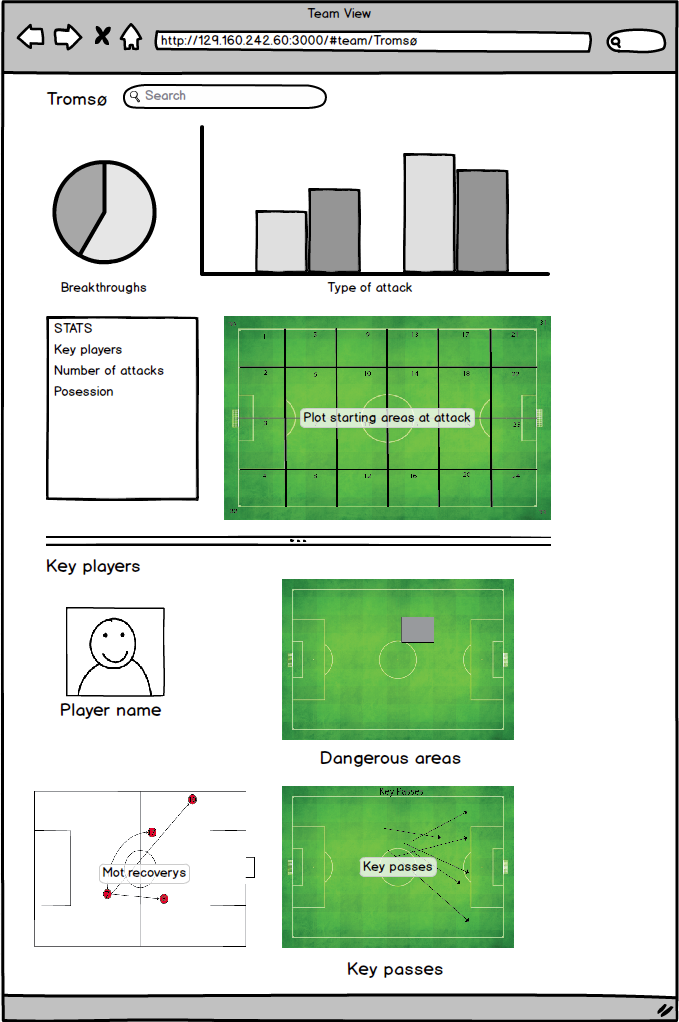
\includegraphics[width=90mm]{images/general/mockup.png}
\caption{A mockup of the main analytic page}
\label{fig:mockup}
\end{figure}

\subsection{Implemented interfaces}

\subsubsection{Home page}
The first page you are prompted with is the listing of all matches registered in the database as figure \ref{fig:all_matches}. A click on match gives you details about that match and prompts you an interface for capturing new attacks if requested. Here you fill out every field in the form.

\begin{figure}[ht!]
\centering
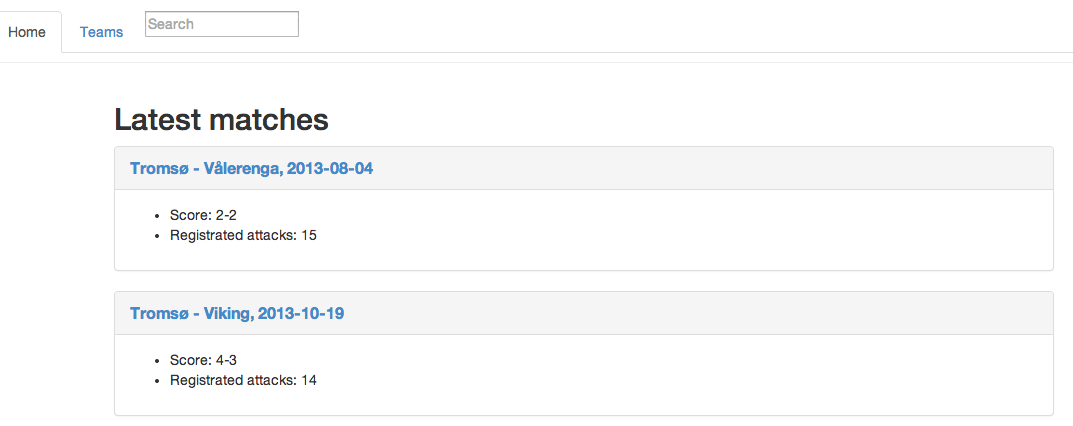
\includegraphics[width=100mm]{images/interfaces/all_matches.png}
\caption{All matches registrated in the database are listed on this page. Image is cropped not listing all matches.}
\label{fig:all_matches}
\end{figure}

Clicking New match sends you to match register interface shown in figure \ref{fig:reg_match}. The users have to register the match he wants to capture data before anything else.

\begin{figure}[ht!]
\centering
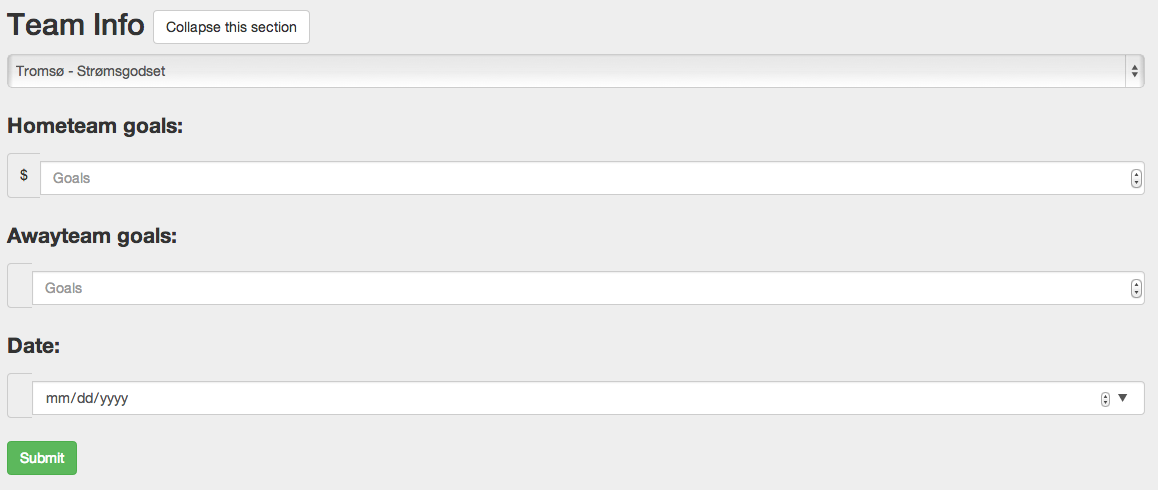
\includegraphics[width=1\textwidth]{images/demo/reg_match.png}
\caption{Interface for registering a match}
\label{fig:reg_match}
\end{figure}


The whole web page follows a theme throughout the pages. This theme is the standard theme in the \ac{CSS} and JavaScript library Bootstrap\footnote{ http://getbootstrap.com/}. Bootstrap makes the website by default responsive. This means the content on the site is automatically re-sized out from your browser window size.


\begin{figure}[ht!]
\centering
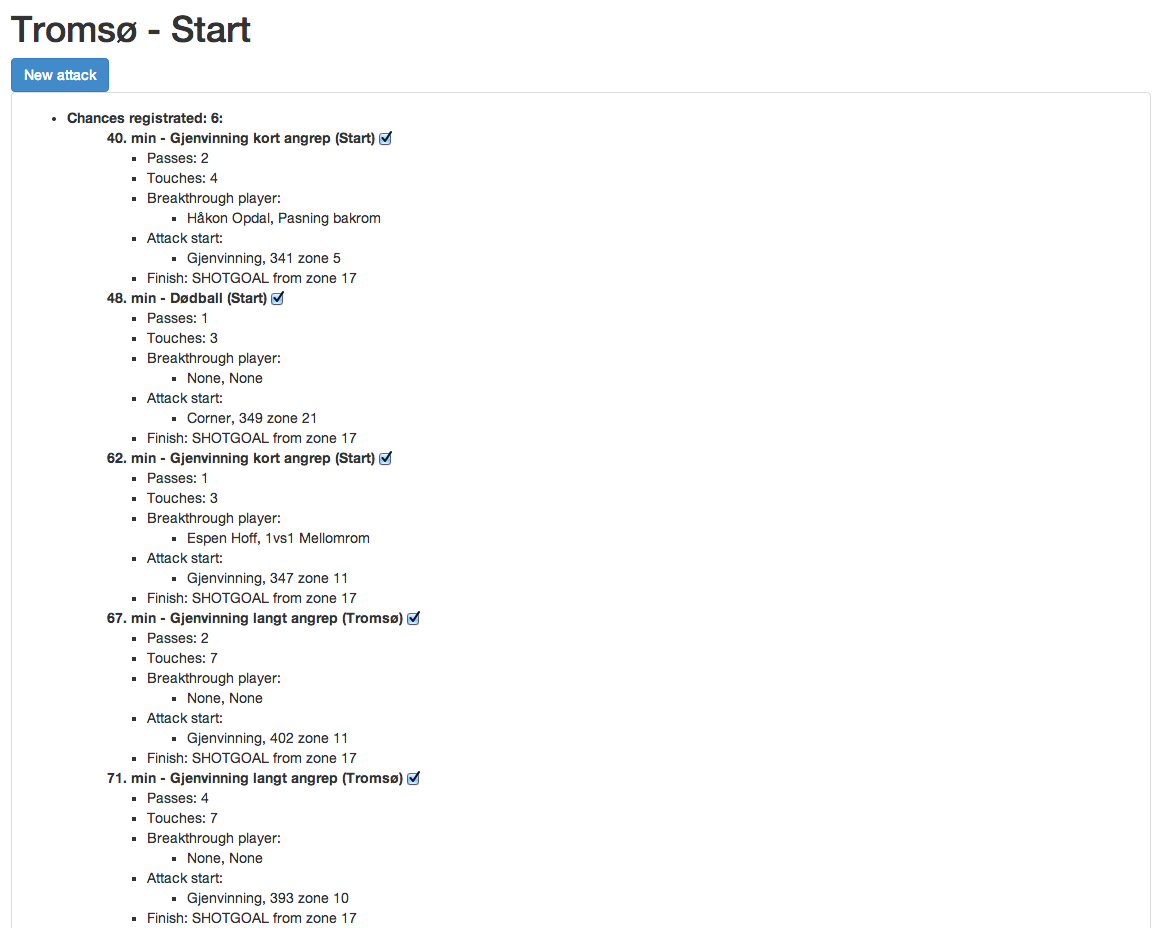
\includegraphics[width=100mm]{images/general/all_attacks.png}
\caption{Interface listing up all attacks for a match.}
\label{fig:all_attacks}
\end{figure}

\subsubsection{Match view}

Clicking on a match gives you overview of all attacks registered for that particular game shown in figure \ref{fig:all_attacks}. This view is only meant for quality checking the data.

From the match page you can add new attack attempts in the interface figure \ref{fig:reg_attack} shows. The user will fill in the form for the attack. Attack start, attack end, breakthrough player, time and team needs to be filled out. The passes in the attack are added by pressing new pass. This will add a new pass to the form. Passes can be deleted by clicking the red remove pass button. 

\begin{figure}[ht!]
\centering
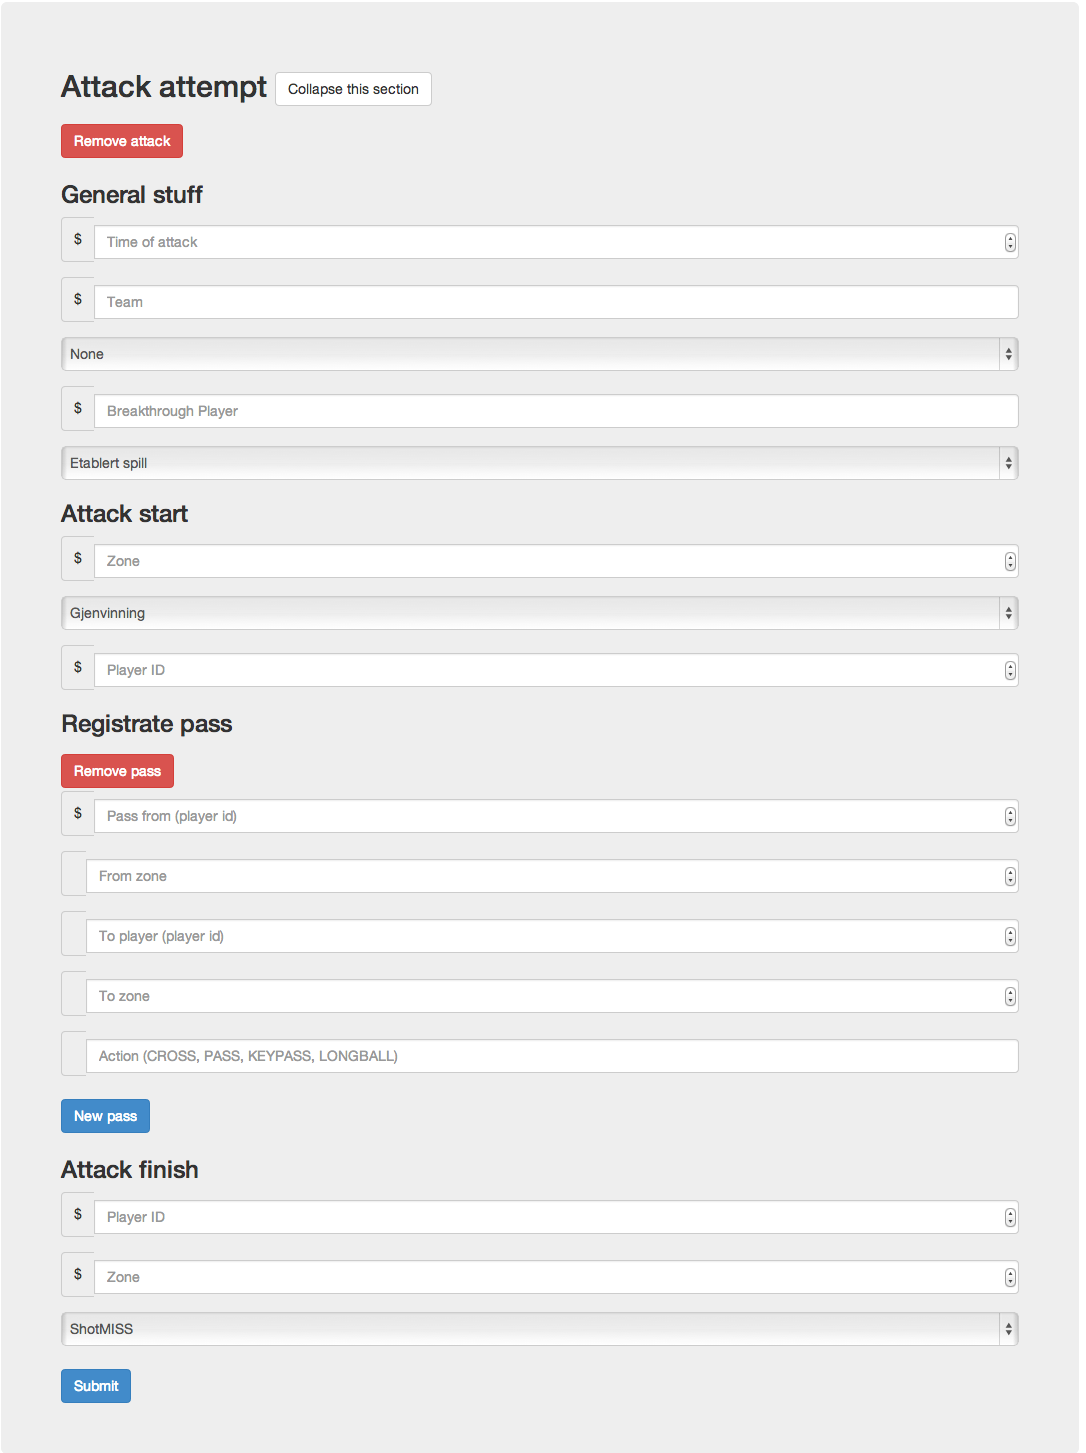
\includegraphics[width=100mm]{images/general/reg_attack.png}
\caption{Interface for register an attack.}
\label{fig:reg_attack}
\end{figure}

\subsubsection{Team view}

Then you have the team selection page shown in figure \ref{fig:all_teams}). This is a simple layout listing all the teams in the Norwegian premier league. From here you select the team you want to analyze.

\begin{figure}[ht!]
\centering
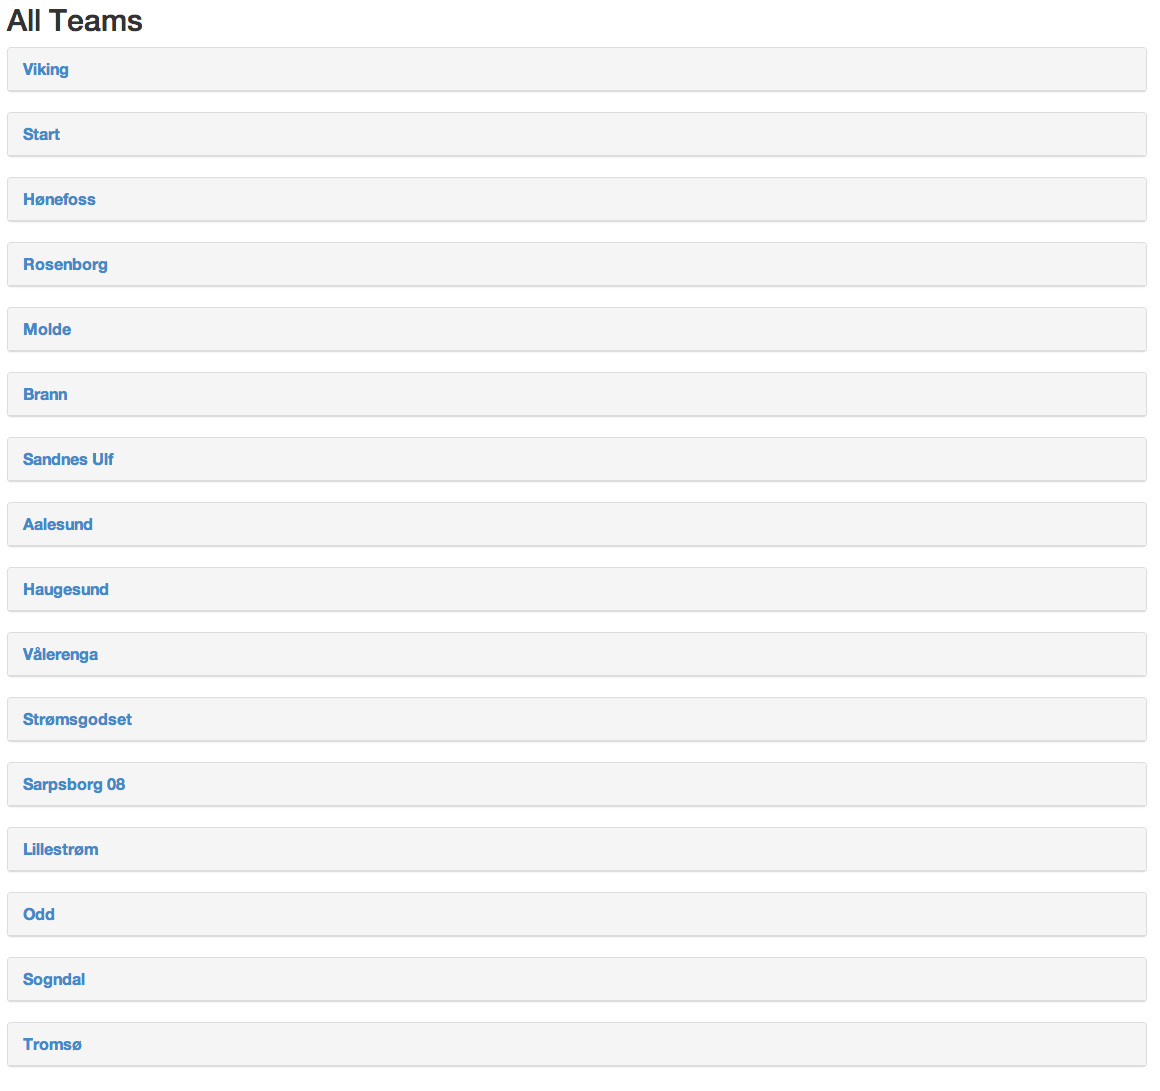
\includegraphics[width=100mm]{images/general/all_teams.png}
\caption{Interface listing all teams.}
\label{fig:all_teams}
\end{figure}

Then there is the main view used for analyzing a team, showed in figure \ref{fig:team_analysis1}, figure \ref{fig:team_analysis2} and figure \ref{fig:team_analysis3}. The page design is not exactly the same as the mockup. This comes from a various things. A description of different breakthroughs has been added to enlighten users of the system. Users of the system may or may not have been involved in the process of capturing the data and therefor-extra information is needed to clarify concepts. In the mockup key players where highlighted. In the final view various statistics is presented to the user and he can then click on players he find interesting to know more about as shown in figure \ref{fig:team_analysis4}. The whole page is divided into 4 sections; key aspects, offensive play, defensive play and players.

\begin{figure}[ht!]
\centering
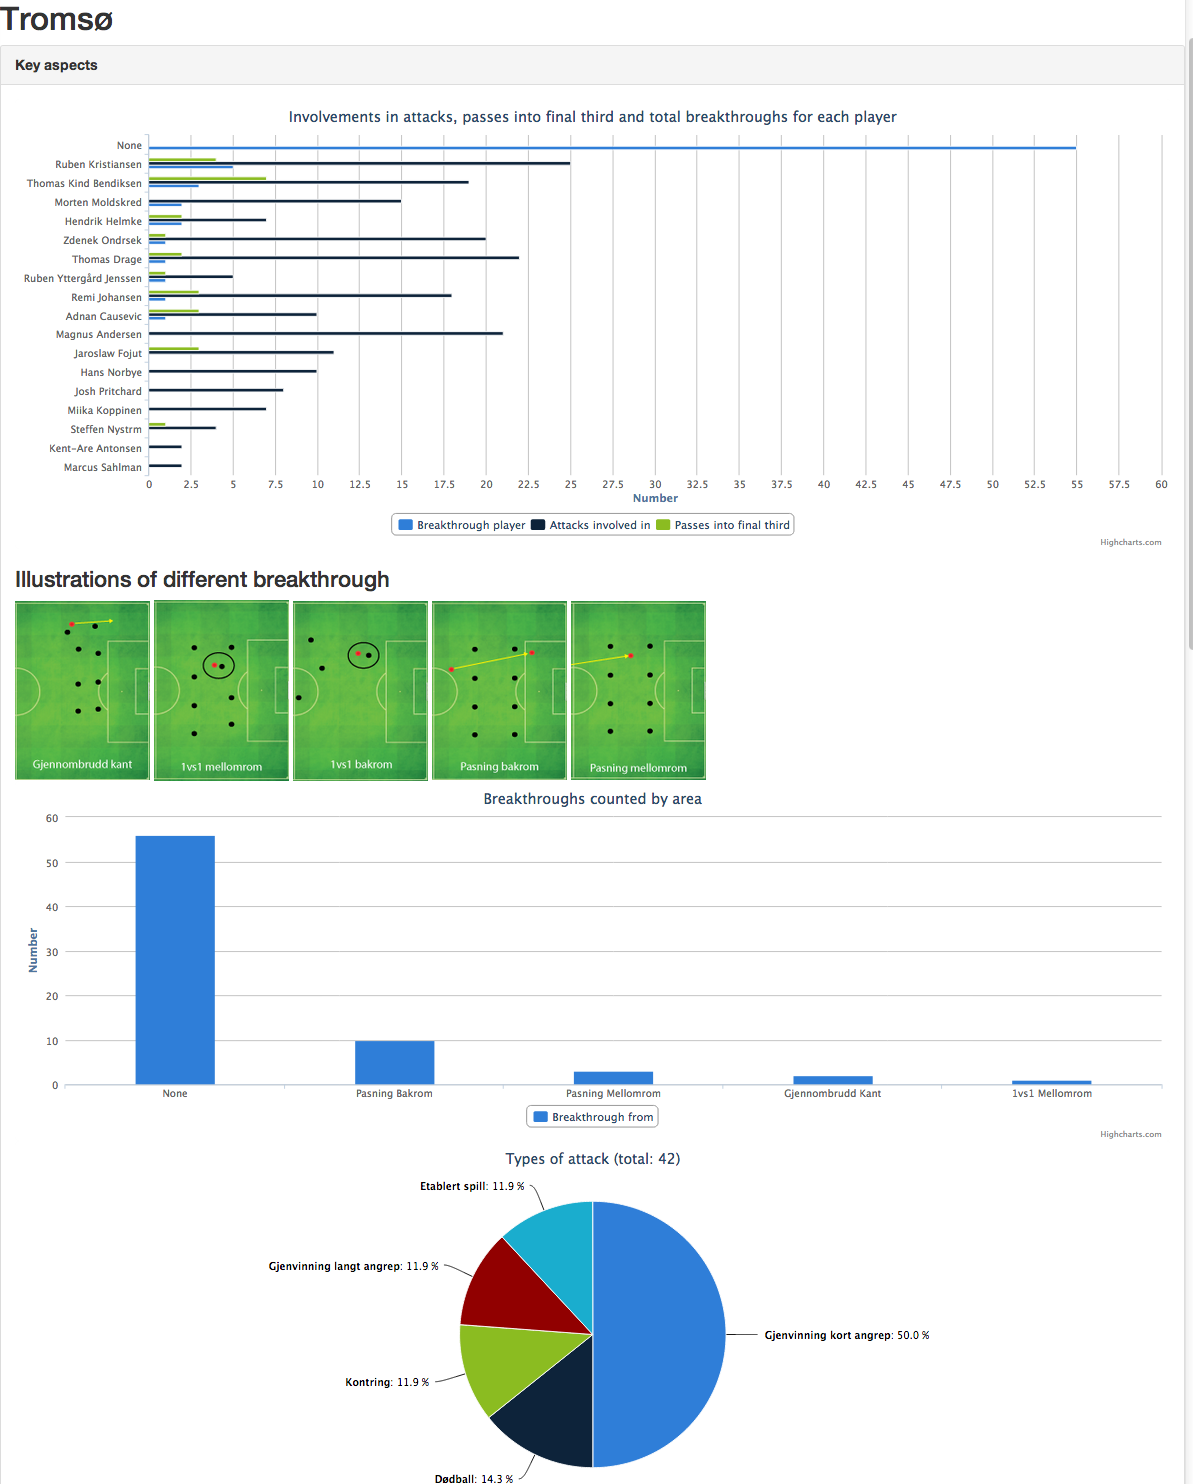
\includegraphics[width=1\textwidth]{images/general/team_analysis1.png}
\caption{Main interface for information about opponents - key aspects.}
\label{fig:team_analysis1}
\end{figure}

\begin{figure}[ht!]
\centering
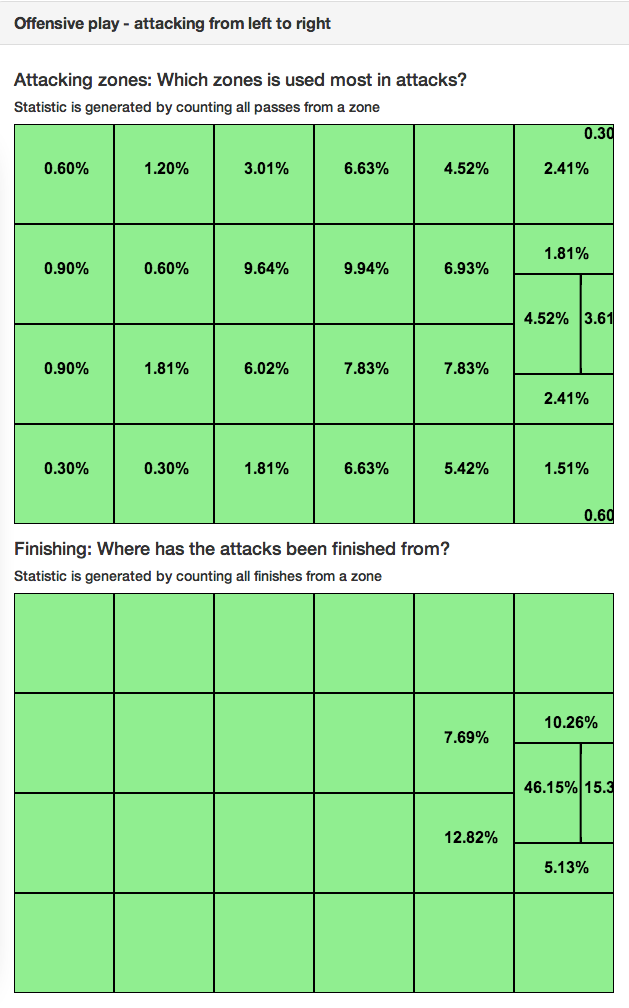
\includegraphics[width=1\textwidth]{images/general/team_analysis2.png}
\caption{Main interface for information about opponents - offensive play.}
\label{fig:team_analysis2}
\end{figure}


\begin{figure}[ht!]
\centering
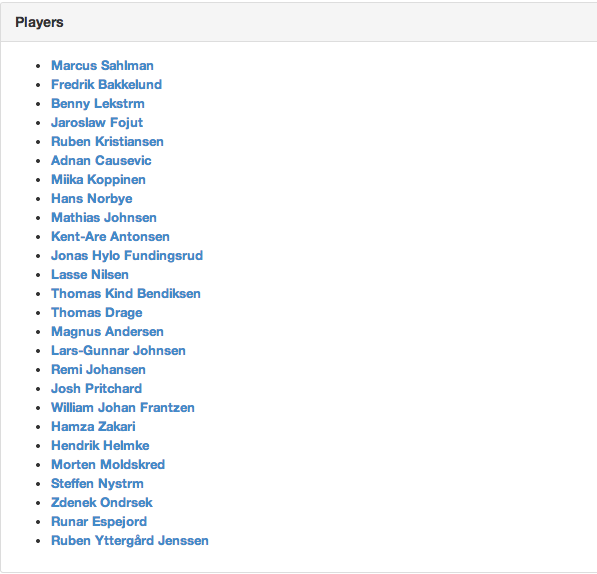
\includegraphics[width=1\textwidth]{images/general/team_analysis3.png}
\caption{Main interface for information about opponents - defensive play.}
\label{fig:team_analysis3}
\end{figure}

\begin{figure}[ht!]
\centering
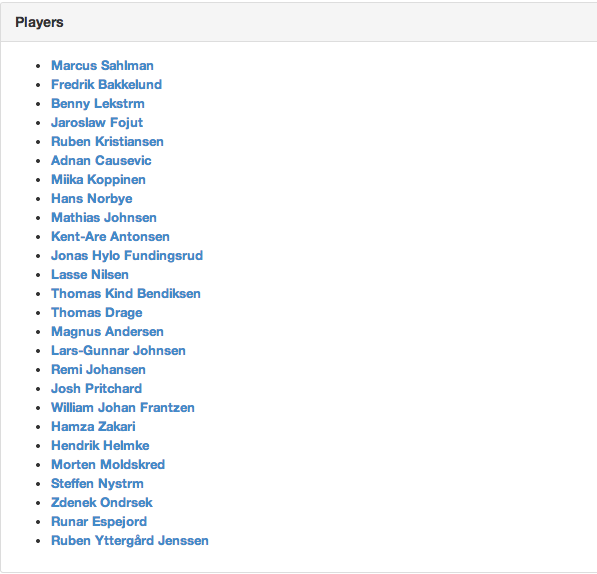
\includegraphics[width=1\textwidth]{images/general/team_analysis4.png}
\caption{All players are listed below the team analytic page. Clicking on a player brings you to the player view.}
\label{fig:team_analysis4}
\end{figure}

\subsubsection{Player view}

Clicking on a player brings you to the player view shown in figure \ref{fig:player_view1} and figure \ref{fig:player_view2}. Here individual statistics is highlighted. 

\begin{figure}[ht!]
\centering
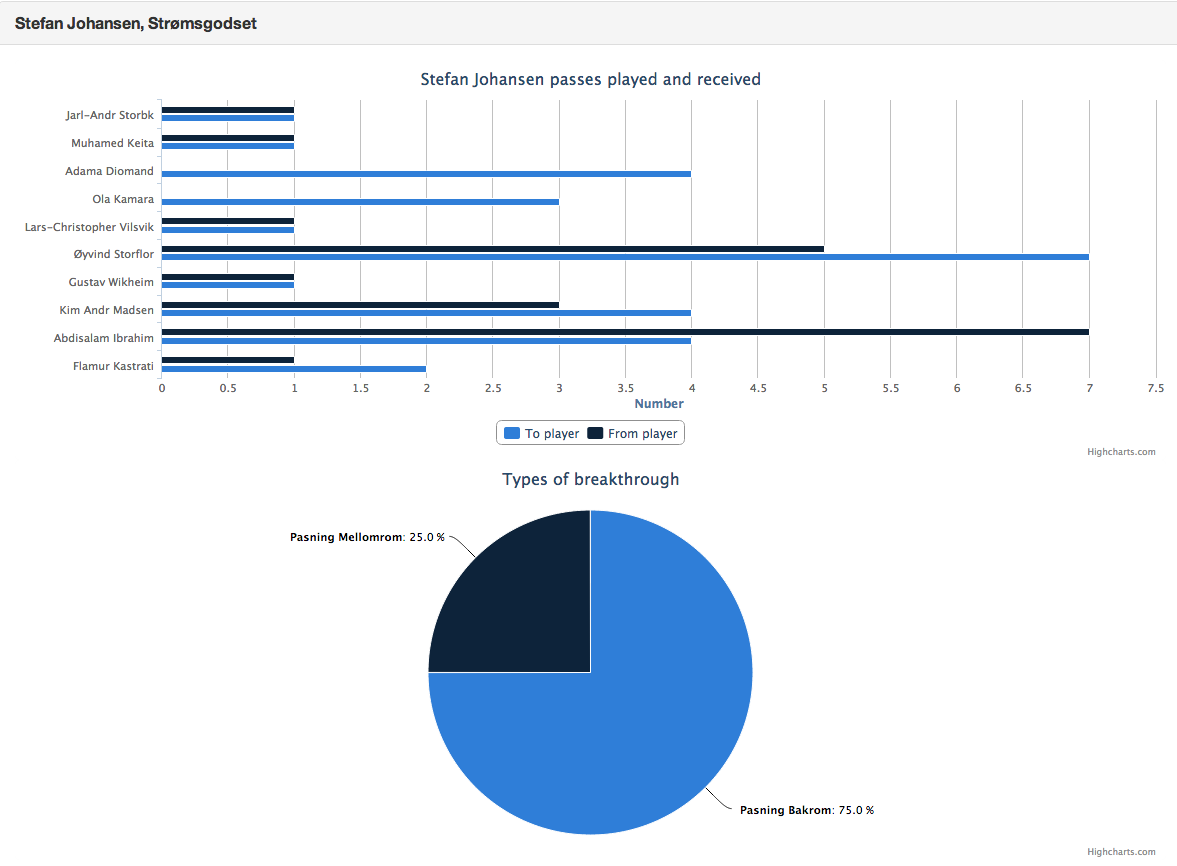
\includegraphics[width=1\textwidth]{images/general/player_view1.png}
\caption{Player view highlighting individual statistics}
\label{fig:player_view1}
\end{figure}

\begin{figure}[ht!]
\centering
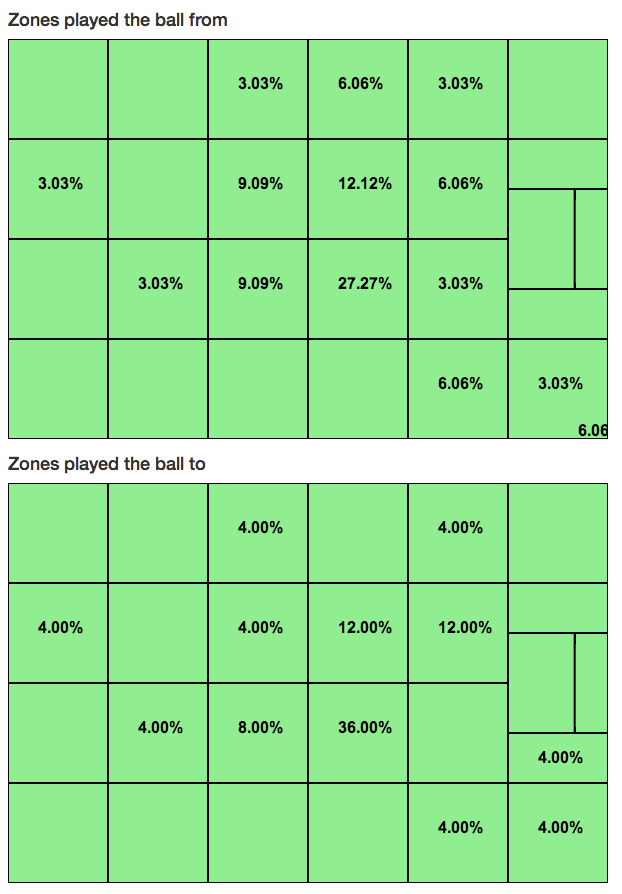
\includegraphics[width=1\textwidth]{images/general/player_view2.png}
\caption{Player view highlighting individual statistics}
\label{fig:player_view2}
\end{figure}


\section{Capturing process}
\label{sec:capprocess}

As mentioned, the process of capturing data is manually. In the beginning it took up to 1 hour to capture all attacks for a match. When you get used to the interface and is able to quickly identify players the time used went down 15-20 minutes. Where most of the time went was getting the players id by looking up in the database manually. To speed up the capturing process the starting 11 names and their corresponding ID where written down with the formation the team plays in to a piece of paper before starting. This also helps identifying players, which can be a bit of a hassle. Match videos came in the resolution 640 * 360 pixels, which is not very good. In addition, on some stadiums there is a running track around the pitch meaning that the grand stands and the main camera is located further away from the pitch. It makes it even harder to identify players on the opposite side of the where the camera is. Having the formation of the team on a paper helps you to identify the players.

The process of capturing has been the following:
\begin{enumerate}
\item Download the match video.
\item Find the match in the VGLive.no archives. VGLive.no is used to quickly find all attacks ending with a finish. Figure \ref{fig:vglive} shows some comments from a match.
\item Register the match by filling out the form in figure \ref{fig:reg_match}.
\item Start finding possible attacks to capture by using VGLive's annotation and jumping in the video. Every event has a time in VGLive.
\item Capture every attack that leads to an attempt on goal one by one via the interface shown in figure \ref{fig:reg_attack}.
\end{enumerate}

\begin{figure}[ht!]
\centering
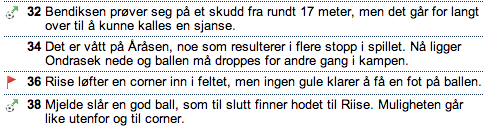
\includegraphics[width=1\textwidth]{images/demo/vglive}
\caption{VGLive.no writes about events in the match. Attempts on goal are tagged with an icon. In the screenshot minute 32 and minute 38 has this icon.}
\label{fig:vglive}
\end{figure}










